%\setcounter{chapter}{-1} % make this chapter 0
\chapter{Introduction}
\label{chap:intro}
%\addcontentsline{toc}{chapter}{Introduction} % but still display in TOC (see https://tex.stackexchange.com/a/222961)

%Inspiration
%\url{https://en.wikipedia.org/wiki/White_dwarf#Formation}
%\url{https://en.wikipedia.org/wiki/Compact_star}

Ever since the dawn of mankind, humans have gazed upon the night sky with great curiosity of what lies beyond our immediate reach.
Not until the Copernican Revolution in the 16th century did we begin to draw a correct picture of how it really looks and where we fit into it.
Nicolaus Copernicus correctly claimed that the Earth revolves around the Sun at the center of a solar system, leading to a number of important discoveries by Tycho Brahe, Johannes Kepler, Galileo Galilei, and culminated in the 17th century as Isaac Newton's described his theory of gravity and motion.
With Newton's theory, humans gained a first scientific understanding of the motion and structure of planets and stars.
During the following scientific revolution, technological advancements in optics and observational techniques made possible not only observation of a number of new stars and planets, but also measurements of their temperature and distance from Earth.
In the 20th century, physicists developed two theories whose application give unprecedented new insight into stars.
First, Albert Einstein's theory of general relativity accurately describes macroscopic aspects of stars where Newton's theory breaks down.
Second, quantum theory developed by physicists like Niels Bohr, Erwin Schrödinger, Werner Heisenberg, Paul Dirac, Enrico Fermi and many others gives us a new understanding of the microscopic properties of stars and their structure.
%Since then, physicists have observed and explained increasingly exotic types of stars.
In this thesis, we will review the fundamental gravitational and quantum theory for studying neutron stars, the smallest and most massive type of star we know of that has not collapsed to a black hole.

\textit{This chapter is inspired by references \cite{ref:glendenning}, \cite{ref:neutron_star_physics}, \cite{ref:lovelace_summary} and \cite{ref:neutron_star_wikipedia}.}

\section{Life, death and structure of stars}

\begin{figure}
\centering
\begin{tikzpicture}[
	edge from parent/.style={draw,very thick,-latex},
	level distance=5cm,
	level 1/.style={level distance=4.1cm},
	level 2/.style={level distance=3.8cm, sibling distance=6.7cm},
	level 3/.style={level distance=4.7cm},
	level 4/.style={level distance=4.3cm, sibling distance=5.3cm},
	sibling distance=6cm,
	every label/.style={text width=4cm, text centered, inner sep=0pt, yshift=+2pt},
	element/.style={font=\small},
	dualpath/.style={
		edge from parent path={(\tikzparentnode\tikzparentanchor) -| (\tikzchildnode\tikzchildanchor)},
	},
	cloud/.pic={
		\node [draw, cloud, element, aspect=2, fill=gray, inner sep=10pt] {H};
	},
	protostar/.pic={
		\node [draw, cloud, aspect=2, fill=black!20!white, inner sep=20pt] {};
		\shade [even odd rule, inner color=black!70!white, outer color=black!20!white] circle (20pt);
		\node [element] at (0, 0) {H};
		\node [element] at (-40pt, 0) {H};
		\node [element] at (+40pt, 0) {H};
	},
	mainsequencestar/.pic={
		\draw[draw=black, fill=orange!50!yellow, circular glow={fill=orange!50!yellow}] circle [radius=30pt]; \node [element] at (90:22.5pt) {H};
		\draw[draw=black, fill=red] circle [radius=15pt]; \node [element] at (90:0pt) {He};
	},
	browndwarf/.pic={
		\filldraw[brown] circle [radius=20pt];
		\node [element] at (90:0pt) {H};
	},
	redgiant/.pic={
		\draw[draw=black, fill=red!75!orange, circular glow={fill=red!75!orange}] circle [radius=40pt]; %\node [element] at (90:30pt) {H};
		\draw[draw=black, fill=orange!50!yellow] circle [radius=30pt]; \node [element] at (90:35pt) {H};
		\draw[draw=black, fill=green!50!gray   ] circle [radius=20pt]; \node [element] at (90:25pt) {He};
		\draw[draw=black, fill=gray            ] circle [radius=10pt]; \node [element] at (90:15pt) {C};
		\draw[draw=black, fill=gray            ] circle [radius= 0pt]; \node [element] at (90: 0pt) {O};
		\draw[draw=none] (-60pt,-60pt) rectangle (+60pt,+60pt);
	},
	redsupergiant/.pic={
		\draw[draw=black, fill=red!75!orange, circular glow={fill=red!75!orange}] circle [radius=50pt]; \node [element] at (90:45pt) {H};
		\draw[draw=black, fill=orange!50!yellow] circle [radius=40pt]; \node [element] at (90:35pt) {He};
		\draw[draw=black, fill=green!50!gray] circle [radius=30pt]; \node [element] at (90:25pt) {$\vdots$ };
		\draw[draw=black, fill=blue!50!gray] circle [radius=20pt]; \node [element] at (90:15pt) {Si};
		\draw[draw=black, fill=gray] circle [radius=10pt]; \node [element] at (90:0pt) {Fe};
		\draw[draw=none] (-60pt,-60pt) rectangle (+60pt,+60pt);
	},
	supernova/.pic={
		\node[starburst, fill=yellow, draw=red, minimum size=2cm] {};
	},
	planetarynebula/.pic={
		\node[starburst, starburst points=14, starburst point height=0.25cm, fill=yellow, draw=red,  minimum size=2.0cm] {};
	},
	blackhole/.pic={
		\draw [fill=black, circular glow={fill=red!50!orange}] circle[radius=40pt];
		\draw[draw=none] (-50pt, -50pt) rectangle (+50pt, +50pt);
	},
	neutronstar/.pic={
		\draw[draw=black, fill=blue!  0!purple, circular glow={fill=blue!0!purple}] circle [radius=45pt]; \node [element, rotate=45] at (135:37.5pt) {H}; \node [element] at ( 90:37.5pt) {$\cdots$}; \node [element, rotate=-45] at (45:37.5pt) {Fe};
		\draw[draw=black, fill=blue! 25!purple] circle [radius=30pt]; \node [element, rotate=+45] at (135:22.5pt) {$n$}; \node [element, rotate=0] at (90:22.5pt) {$p$}; \node [element, rotate=-45] at (45:22.5pt) {$e^-$};
		\draw[draw=black, fill=blue! 50!purple] circle [radius=15pt]; \node [element] at (90:0pt) {???};
		\draw[draw=none] (-50pt, -50pt) rectangle (+50pt, +50pt);
	},
	whitedwarf/.pic={
		\draw[draw=black, fill=white!80!gray, circular glow={fill=cyan! 20!white}] circle [radius=30pt]; \node [element, rotate=+30] at (120:22.5pt) {H}; \node [element, rotate=-30] at (60:22.5pt) {He};
		\draw[draw=black, fill=cyan!60!white] circle [radius=15pt]; \node [element] at (90:0pt) {C  O};
		\draw[draw=none] (-50pt, -50pt) rectangle (+50pt, +50pt);
	},
]

	\node (protostar) {\tikz \node [label={[text width=6.0cm]below:\subcaption{\label{fig:intro:star_evolution_protostar}protostar in giant molecular cloud}}] {\tikz \pic {protostar};};}
		child { node [label={[]below:\subcaption{\label{fig:intro:star_evolution_mainseq}main sequence star}}] {\tikz \node [] {\tikz \pic {mainsequencestar};};}
			child { node {\tikz \node [label={below:\subcaption{\label{fig:intro:star_evolution_red_giant}red giant}}] {\tikz \pic {redgiant};};}
				child { node (planetarynebula) {\tikz \node [label={below:\subcaption{\label{fig:intro:star_evolution_planetary_nebula}planetary nebula}}] {\tikz \pic {planetarynebula};};}
					child { node {\tikz \node [label={below:\subcaption{\label{fig:intro:star_evolution_white_dwarf}white dwarf}}] {\tikz \pic {whitedwarf};};} }
				} edge from parent [dualpath] node [above, anchor=south west, xshift=-2pt] {$M \lesssim 8 \solarmass$}
			}
			child { node {\tikz \node [label={below:\subcaption{\label{fig:intro:star_evolution_red_supergiant}red supergiant}}] {\tikz \pic {redsupergiant};};}
				child { node (supernova) [label={below:\subcaption{\label{fig:intro:star_evolution_supernova}supernova}}] {\tikz \node [] {\tikz \pic {supernova};};}
					child { node {\tikz \node [label={below:\subcaption{\label{fig:intro:star_evolution_neutron_star}neutron star}}] {\tikz \pic {neutronstar};};} edge from parent [dualpath] node[above, anchor=south west, xshift=-8pt] {$M \lesssim 40 \solarmass$} }
					child { node {\tikz \node [label={below:\subcaption{\label{fig:intro:star_evolution_black_hole}black hole}}] {\tikz \pic {blackhole};};} edge from parent [dualpath] node[above, anchor=south east, xshift=+8pt] {$M \gtrsim 40 \solarmass$} }
				}
				edge from parent [dualpath] node [above, anchor=south east, xshift=+2pt] {$M \gtrsim 8 \solarmass$}
			}
		};
	\draw [-latex, dashed] (supernova)       to [out= 45, in=  0, out looseness=0.5] (protostar);
	\draw [-latex, dashed] (planetarynebula) to [out=135, in=180, out looseness=0.5] (protostar);
\end{tikzpicture}
\caption{\label{fig:intro:star_evolution}%
	Simplified life cycle of stars and their main structure at every stage (not to scale).
}
\end{figure}

% planetary nebula -> releases ionized gas -> forms clouds
The mother of any star is an enormous accumulation of light elements called a \textbf{giant molecular cloud}.
Such clouds consist predominantly of hydrogen and some helium produced in the nucleosynthesis that followed the Big Bang.
In addition, there are trace amounts of heavier elements from the ashes of dying stars at the end of the life cycle we have just begun to describe.
They can contain millions of solar masses distributed over a huge region hundreds of lightyears across with a relatively low average density.
Internally, the dynamics of a molecular cloud is chiefly governed by a balance between the attractive force of gravity between particles and the repulsive thermal pressure from their motion and collisions.

Due to the force of gravity, parts of the cloud can clump together in regions of greater density.
As more mass accumulates, the force of gravity attracting the surrounding material only increases, causing a snowball effect that amplifies the growth of the clump.
Initially, the clump is not so dense, and thermal radiation can escape to the outside, resulting in low temperatures and pressure and allowing the clump to contract with little resistance.
However, once the density reaches a sufficiently high level, the clump becomes opaque and traps the thermal radiation inside.
When this happens, the temperature increases, in turn increasing the outwards pressure counteracting the inwards gravitational collapse, thus considerably slowing down the contraction.
During this stage, as the child ``clump'' grows by sucking up material from its parent cloud, it receives the honorable name \textbf{protostar} (\cref{fig:intro:star_evolution_protostar}).

Sooner or later, the protostar has depleted the cloud of its available mass and is promoted to a \textbf{pre-main-sequence star}.
Whatever total mass $M$ has been gathered by now will determine the fate of the star for the rest of its life.
The contraction continues until the temperature and pressure have increased sufficiently for the star to reach a state of equilibrium.
Provided that the protostar has accumulated at least $M \gtrsim 0.08 \solarmass$, the temperature will reach $T \gtrsim \SI{1e7}{\kelvin}$ -- sufficient for the fusion of hydrogen into helium to take place.
The ignition of hydrogen marks the transition into a \textbf{main sequence star} (\cref{fig:intro:star_evolution_mainseq}).
For billions of years, the star supports itself in this state by burning hydrogen into helium.
As time goes on, the hydrogen in the central region is depleted, leaving behind a helium \emph{core} surrounded by a hydrogen \emph{envelope}.

What happens once there is no more hydrogen that can burn depends heavily on the mass of the star.
Stars up to $M \lesssim 8 \solarmass$ evolve into \textbf{red giants} (\cref{fig:intro:star_evolution_red_giant}).
As the hydrogen is exhausted, the pressure falls and fails to support the star, so the core begins to contract again, in turn causing another increase in temperature.
For heavier red giants, the temperature can increase to $T \gtrsim \SI{1e8}{\kelvin}$, activating both fusion of helium to carbon and carbon to oxygen, but not of heavier elements.
As these processes take place and the burning of each element successively finishes, the core develops shells with elements of increasing mass towards the center as shown in the figure, from hydrogen to helium, carbon or oxygen, depending on the exact mass of the star.
Due to the sudden increase in temperature, much energy is transported into the envelope, where it reignites leftover hydrogen and inflates the envelope up to 200 solar radii.

Eventually, explosions in the envelope of a red giant trigger unstable pulsations of the hydrogen envelope.
This causes a \textbf{planetary nebula} (\cref{fig:intro:star_evolution_planetary_nebula}) -- an ejection of the outer shells of the red giant into new clouds from which new stars are born.
The remaining inert core that is left intact from the nebula forms a \textbf{white dwarf} (\cref{fig:intro:star_evolution_white_dwarf}).
Since no further reactions occur in the core, it is supported against collapse solely by degeneracy pressure of electrons that are ripped away from the arms of their parent atoms at high density and forced to occupy different states by the Pauli exclusion principle.
White dwarfs can be as hot as $T \approx \SI{1e7}{\kelvin}$ upon formation, but gradually cool down as they radiate away their energy.
%Importantly, Chandrasekhar derived that ideal white dwarfs consisting of a relativistic degenerate electron gas can only support themselves for masses up to $M \lesssim 0.91\solarmass$. \cite{ref:chandrasekhar_limit_ideal} \TODO{ideal}
%A few years later, he took more effects into account and derived the more accurate Chandrasekhar limit $M \lesssim 1.47$. \cite{ref:chandrasekhar_limit_nonideal}
Importantly, Chandrasekhar showed that white dwarfs can only support masses up to $M \lesssim 1.47 \solarmass$. \cite{ref:chandrasekhar_limit_nonideal}
He modelled the interior as a relativistic Fermi gas of protons, neutrons and electrons and demonstrated that virtually all the pressure that prevents collapse comes from the degeneracy of the electrons, while the protons and neutrons contribute most of the energy density due to their much greater mass.
In his honor, the true upper mass limit of white dwarfs is named the Chandrasekhar limit and is currently believed to be closer to $M \lesssim 1.44 \solarmass$. \cite{ref:glendenning}

\begin{figure}
\centering
%\includesvg[width=0.6\textwidth]{figures/binding_energy_curve.svg}
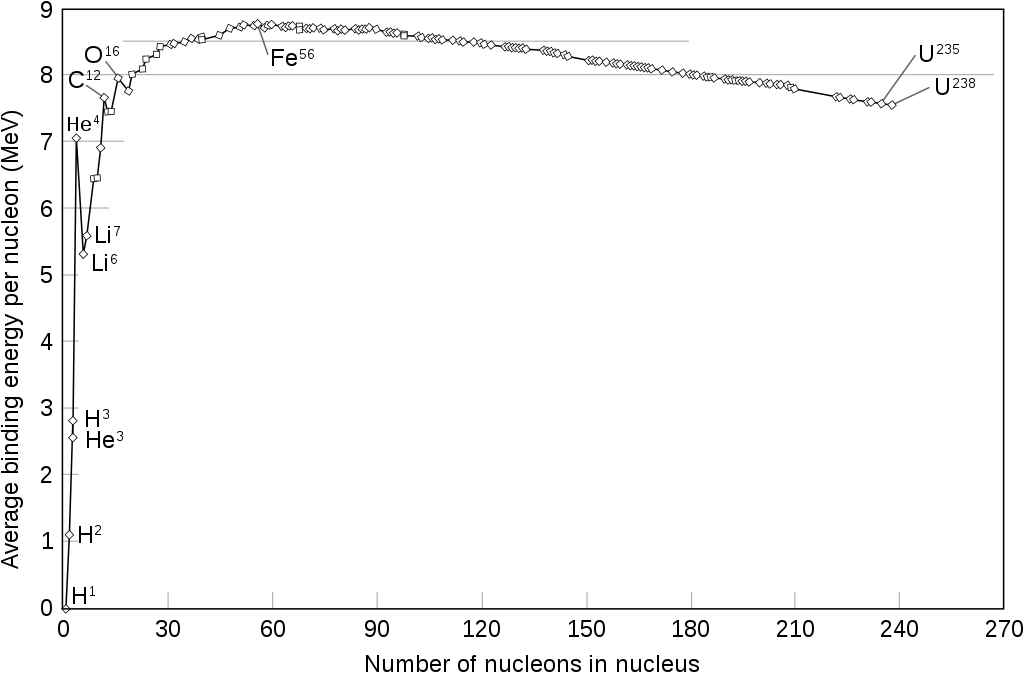
\includegraphics[width=0.6\textwidth]{figures/binding_energy_curve.png}
\caption{\label{fig:intro:iron_peak}%
	The binding energy per nucleon displays a peak near iron.
	From \cite{ref:wiki_iron_peak_figure}
}
\end{figure}

If the mass of a main sequence star exceeds $M \gtrsim 8 \solarmass$, it first becomes a more intense red giant -- a \textbf{red supergiant} (\cref{fig:intro:star_evolution_red_supergiant}), for lack of a better word.
The increased mass sends the temperature soaring well above $T \gtrsim \SI{1e8}{\kelvin}$, activating not only fusion from hydrogen to helium, carbon and oxygen, but even to heavier elements such as neon and iron.
When the reactions reach iron, something dramatic happens.
As shown in \cref{fig:intro:iron_peak}, fusion from lighter elements \emph{release} energy, while fusion from iron or heavier elements \emph{require} energy, causing the burning to stop at iron.
At this point, due to the heavy elements, the core of a red supergiant is so massive that it exceeds the Chandrasekhar limit.
Inevitably, the core collapses and produces an extremely powerful explosion called a \textbf{supernova} (\cref{fig:intro:star_evolution_supernova}).

For supergiants whose mass does not exceed $M \lesssim 40 \solarmass$, the supernova leaves behind an inert core called a \textbf{neutron star} (\cref{fig:intro:star_evolution_neutron_star}).
The core is then too massive that it is compressed \emph{past} the Chandrasekhar limit of white dwarfs.
The resulting extreme density and Fermi energy makes it energetically favorable for electrons and protons to combine into neutrons in inverse beta decay.
In general, the outer core of a neutron star can consist of a neutron ($n$) superfluid mixed with superconducting protons ($p$), electrons ($e^-$) and muons ($\mu^-$). % Potekhin section 2.2
The precise composition of the inner core is an open question, but it is believed that it may contain $\lambda$ and $\Sigma^-$ baryons, $\pi$ and $K$ mesons and deconfined quark matter. % Potekhin section 2.2 list 1-4
Thus, compact stars are not only imporant for astrophysics as an isolated field, but also serve as a testbed for nuclear and particle physics.
Outside the core, there is an envelope consisting of more ``ordinary'' matter with isolated atomic nuclei, such as iron. % Potekhin 2.2 last paragraph
%making a neutron star consist protons, hyperons, leptons and possibly quarks. % Glendenning somewhere
Despite their differences, all the particles group up for a last stand against gravity, reaching a new equilibrium configuration that is known as a neutron star.
As with white dwarfs, there is a limit for the gravitational force that their degeneracy pressure can withstand.
Assuming a neutron star consists of an ideal Fermi gas of pure neutrons, Oppenheimer and Volkoff computed the mass bound $M \lesssim 0.7 \solarmass$ in 1939, building upon earlier work by Tolman. \cite{ref:tov,ref:tolman}
More advanced theories and observations place the so named Tolman-Oppenheimer-Volkoff limit for the maximum mass of real neutron stars somewhere between $2 \solarmass$ and $3 \solarmass$. % Potekhin section 2.3
Like white dwarfs, neutron stars only cool down by radiating their stored energy, from initial core temperatures $T \approx \SI{1e10}{\kelvin}$ to $T \approx \SI{1e8}{\kelvin}$ in a month, then to $T \approx \SI{1e6}{\kelvin}$ in less than a million years. \cite{ref:glendenning} % Glendenning page 115

Finally, for even more massive supergiants with $M \gtrsim 40 \solarmass$, the Oppenheimer-Volkoff limit is exceeded, and not even the degeneracy pressure of neutrons can resist gravity.
Beyond this limit, no known star has escaped the collapse to a \textbf{black hole} (\cref{fig:intro:star_evolution_black_hole}).
It is, however, an open question whether there can be even more classes of stars that fall between the Oppenheimer-Volkoff limit and the lightest observed black holes.
No such stars have been observed yet, and they are therefore referred to as \textbf{exotic stars}, of which \textbf{quark stars} is one example.

This marks the last possible path of evolution in the somewhat simplified diagram in \cref{fig:intro:star_evolution}.
Notably, we ignored the possibility that main sequence stars with $M \lesssim 0.08 \solarmass$ never reach the temperature necessary to ignite hydrogen and become \textbf{brown dwarfs}.

\section{Proposition and observation of neutron stars}

Only two years after James Chadwick discovered the neutron in 1932, \cite{ref:neutron_discovery}
Walter Baade and Fritz Zwicky proposed the existence of stars composed of them.
At the time, physicists had only recently begun to study supernovas and the origin of cosmic rays.
In developing an explanation of the detailed mechanisms involved in a supernova, they suggested -- with great accuracy -- that
\cite[page 263]{ref:supernova_cosmic_rays_neutron_stars}
\begin{displayquote}
(...) %With all reserve we advance the view that
a super-nova represents the transition of an ordinary star into a \emph{neutron star}, consisting mainly of neutrons.
Such a star may possess a very small radius and an extremely high density.
As neutrons can be packed much more closely than ordinary nuclei and electrons, the ``gravitational packing'' energy in a cold neutron star may become very large, and, under certain circumstances, may far exceed the ordinary nuclear packing fractions.
A neutron star would therefore represent the most stable configuration of matter as such.
\end{displayquote}

\iffalse
The first theoretical model of a neutron star was developed by Oppenheimer and Volkoff in 1939. \cite{ref:tov}
Assuming a neutron star consists entirely of a non-interacting cold Fermi gas, they found an equation of state governing its internals and solved the Einstein field equations in a radially symmetric perfect fluid to find the mass and radii of neutron stars.
In such a cold gas, thermal motion contributes nothing to the pressure, so any pressure is only due to the Pauli exclusion principle, stating that no fermions can be in the same quantum state.
Analogously to the Chandrasekhar limit, their results implied that this degeneracy pressure could only support masses up to $M < 0.7 \solarmass$.
\fi

% see https://en.wikipedia.org/wiki/Pulsar
Up until the late 1960s, the existence of neutron stars was only considered a theoretical possibility.
How \emph{on Earth} would one ever detect such an object, given their assumed small size, rarity and faint thermal radiation?
It was first in 1968 that Jocelyn Bell, a PhD student of Antony Hewish, recorded an unusual \textbf{pulsa}ting \textbf{r}adio signal from an extraterrestial source, now referred to as a \textbf{pulsar}. \cite{ref:neutron_star_discovery_first}
The signal consisted of short, Gaussian pulses lasting about \SI{0.3}{\second} each, repeating themselves with extreme accuracy with a period of \SI{1.337}{\second}.
At first, it was speculated that the source could be a white dwarf oscillating radially at the corresponding frequency.
Thomas Gold provided an alternative explanation, suggesting the signal arose from a \emph{rotating} neutron star with a strong magnetic field. \cite{ref:neutron_star_gold}
He imagined the star's magnetic field to be reminiscent of a dipole and that a directional signal was emitted from localized spots on the star corresponding to the magnetic poles.
This picture naturally explained the Gaussian shape of the short pulses, as one would detect a similar pattern by measuring the intensity of a directed, rotating lighthouse beam from a fixed position.
In contrast, radial pulsations did not explain the shape nor the extreme regularity of the signal.
Not long after, Richard Lovelace and others measured a similar signal from the pulsar NP 0532 in the Crab Nebula -- also referred to as the Crab Pulsar -- with a period of only \SI{33}{\milli\second}, which was even more challenging to explain by radial oscillations. \cite{ref:crab_pulsar_period_discovery}
Moreover, David Richards discovered that the period slightly increased with time in the way that it should for a rotating object that radiates away its energy.
This evidence convinced physicists that the signals were indeed from real, rotating and pulsating \textbf{neutron stars}.
Controversially, Bell's supervisor and first author Hewish later got the Nobel prize for the discovery of the neutron star, although it was Jocelyn who made the actual measurements and in hindsight credited first.


\section{Outline of this thesis}

In this thesis, we first develop the fundamental theoretical tools that are necessary to study neutron stars.
Then we apply them to calculate masses and radii of neutron stars and study the stability of these stars.

In \textbf{\cref{chap:intro}}, you already know that we have presented the life cycle of stars and the history of the proposition and discovery of neutron stars.

In \textbf{\cref{chap:tov}}, we derive the \textbf{Tolman-Oppenheimer-Volkoff system of equations}
\begin{align*}
	\odv{P}{r} &= -\frac{G m \epsilon}{r^2 c^2} \left( 1 + \frac{P}{\epsilon} \right) \left( 1 + \frac{4 \pi r^3 P}{m c^2} \right) \left( 1 - \frac{2 G m}{r c^2} \right)^{-1} , \\
	\odv{m}{r} &= \frac{4 \pi r^2 \epsilon}{c^2} ,
	%\odv{\alpha}{r} &= -\frac{1}{\epsilon(P)+P} \odv{P}{r} ,
\end{align*}
from the Einstein field equations of general relativity.
This is a system of two differential equations for the unknown pressure $P(r)$, mass $m(r)$ and energy density $\epsilon(r)$ at radius $r$ from the center of a star composed of a \emph{perfect fluid} in \emph{equilibrium}.
An additional equation of state $\epsilon = \epsilon(P)$ that allows computation of the energy density corresponding to a given pressure is needed to solve the system.
This is outside the scope of general relativity and belongs to the field of quantum theory and statistical mechanics.
Given the equation of state, however, one may impose the boundary condition $m(0) = 0$ and any central pressure $P(0) = P_c$ and solve the system for the pressure profile $P(r)$ and mass profile $m(r)$ in the star.
By defining the surface $r=R$ of the star where the pressure $P(R) = 0$ vanishes, one can obtain the radius $R$ and mass $M = m(R)$ of the star.
In particular, we will solve the system analytically for a star of constant energy density $\epsilon(P) = \epsilon_0$ to derive the Buchdal limit
\begin{equation*}
	\frac{M}{R} < \frac{4 c^2}{9 G}
\end{equation*}
on the mass-radius ratio of \emph{any} star.

In \textbf{\cref{chap:tft}}, we will study \textbf{thermal field theory} -- the formalism needed to find the effects of quantum fields at nonzero temperature.
We will show how to write the quantum partition function
\begin{equation*}
	Z = \trace \left[ e^{-\beta(\hat{H} - \mu_i \hat{N}_i)} \right]
\end{equation*}
as a path integral.
First, we use the path integral to find the partition function of a gas of free bosons.
Next, we introduce Grassmann numbers and fermionic coherent states to derive a path integral that is valid for fermions, and calculate it for a free Fermi gas.
From this partition function, we can calculate the energy density and pressure and hence the equation of state.

In \textbf{\cref{chap:nstars}}, we put together the pieces of \cref{chap:tov} and \cref{chap:tft} and study \textbf{ideal neutron stars} made of a \textbf{cold free Fermi gas}.
From the partition function $Z$ of \cref{chap:tft}, we find the equation of state
\begin{equation*}
	\epsilon = \epsilon(P)
\end{equation*}
for the Fermi gas at zero temperature.
We then solve the Tolman-Oppenheimer-Volkoff equation numerically for this equation of state to find a mass-radius curve $[R(P_c), \, M(P_c)]$ for such stars parametrized by their central pressure.
Finally, we study whether stars on the curve are in stable or unstable equilibrium.
We begin by establishing a set of necessary criteria from simple physical considerations.
Then we develop a mathematically rigorous criterion for the stability of stars by using perturbation theory on the equilibrium Einstein field equations in \cref{chap:tov} to study the behavior of the perfect fluid as it is disturbed from equilibrium.
This results in a Sturm-Liouville problem for normal vibration modes $U_n(r)$ with squared frequencies $\omega_n^2$ whose sign determine whether an exponential time dependence $e^{i \omega_n t}$ on the motion of disturbed fluid elements oscillate or grow exponentially.

In \textbf{\cref{chap:conclusion}}, we \textbf{conclude} by \textbf{discussing} our results in light of observations and presenting an \textbf{outlook} on more advanced theories of neutron stars.

In \textbf{\cref{chap:gr}}, we give a comprehensive \textbf{review of the theory of general relativity}.
Here, we derive the Einstein field equations from the principle of least action and cover all aspects of general relativity that we require for \cref{chap:tov} and \cref{chap:nstars}, including a detailed discussion of the Newtonian limit.

In \textbf{\cref{chap:relfluid}}, we briefly summarize \textbf{relativistic fluid mechanics} for a perfect fluid.
Here, we derive relativistic generalizations of results from ordinary fluid mechanics, such as the Euler equation and the equation of energy conservation.
These results are needed to understand the behavior of fluids out of equilibrium in the stability analysis in \cref{chap:nstars}.

In \textbf{\cref{chap:matsum}}, we describe the technique of \textbf{Matsubara frequency summation}.
This is an elegant mathematical tool that allows us to compute a general class of infinite sums we encounter in \cref{chap:tft}.
Despite their purely mathematical foundation, the results of this appendix naturally give rise to the Bose-Einstein and Fermi-Dirac distributions, and are therefore of great physical interest, too.

In \textbf{\cref{chap:integrals}}, we give concise derivations of all \textbf{integrals} used throughout this thesis.
Whenever we encounter difficult integrals in the main text, we will always write the result directly and refer back to this appendix for readers who wish to investigate them in more detail.

In \textbf{\cref{chap:code}}, we describe implementations of \textbf{numerical methods and algorithms}.
Here, we present dimensionless forms of the TOV equations in \cref{chap:tov} and the equations of stellar instability in \cref{chap:nstars}, and show how they can be solved with Runge-Kutta methods and the shooting method, respectively.
